\section{任务1\quad 图像无监督聚类}
\label{sec:task1}
\subsection{问题描述与定义}
设课程图像集合为 $\mathcal X=\{x_i\}_{i=1}^{600}$。题目给定簇数 $K=6$，求互不重叠且覆盖 $\mathcal X$ 的非空簇 $\{C_k\}_{k=1}^K$。簇编号可任意置换，算法不使用类别名称、逐图类别标签或每簇容量约束。每图输出簇编号 $z_i\in\{1,\ldots,K\}$。训练阶段只读取像素，图结构和超参数据此确定。课程标签文件仅在评估阶段读入。

\subsection{图像特征表示}
将图像转成 RGB，用双线性插值缩放到 $224\times224$。输入网络前用 ImageNet 通道均值 $(0.485,0.456,0.406)$ 与标准差 $(0.229,0.224,0.225)$ 归一化，冻结 ImageNet 预训练的 ResNet-50（\texttt{IMAGENET1K\_V2} 权重）\cite{he2016,torchvisionweights}。卷积与池化的作用可参照课程第6章\cite{coursedeep}。将 \texttt{layer3}、\texttt{layer4} 的每个通道做全局均值池化，保留瓶口、药片等物体的整图信息。用 \texttt{layer2}、\texttt{layer3} 的通道标准差描述特征响应的空间起伏。颜色块由每通道 16 桶的归一化直方图和 $8\times8$ 网格的分块 RGB 均值组成，可补充皮革和瓷砖等类别的外观差异。

按课程特征工程中尺度归一化的思路\cite{coursefeat}，对每个非负块先逐元素开平方，再做 $\ell_2$ 归一化，记作 $\widehat{\vect f}_b$。拼接时用 $\sqrt{w_b}$ 缩放，得到
\begin{equation}
 \vect z=[\sqrt{w_b}\,\widehat{\vect f}_b]_b,
 \qquad
 \|\vect z_i-\vect z_j\|_2^2
 =\sum_b w_b\|\widehat{\vect f}_{ib}-\widehat{\vect f}_{jb}\|_2^2 .
\end{equation}
五块权重依次为 $0.32,\ 0.48,\ 0.08,\ 0.07,\ 0.05$，对应两个均值块、两个标准差块和颜色块，共 4\,848 维。均值块占八成，以整图语义为主。纯深度对照只使用两个均值块，权重为 $0.4$ 和 $0.6$。手工对照使用颜色块和灰度差分，两者权重为 $0.8$ 和 $0.2$。差分在横向和纵向各取间隔 $1,2,4,8,16$ 像素，汇总每组绝对差值的均值和标准差，再逐维标准化并按行归一化。

\subsection{方法}
物体、材料纹理和拍摄背景各有变化。全局 K-means 依赖样本到质心的距离，谱聚类则可以沿近邻图发现由多段局部邻域连成的簇。在本实验中，用两点间欧氏距离 $d_{ij}$ 寻找每图的 $h$ 个近邻。若一方是另一方的近邻，就保留这条无向边。参考局部尺度核\cite{zelnik2004}，以样本到第 $h$ 个近邻的距离为 $\sigma_i$，令
\begin{equation}
 W_{ij}=\exp\!\left(
    -\frac{d_{ij}^2}{\max(\sigma_i,\epsilon)\max(\sigma_j,\epsilon)}
                         \right),
\end{equation}
其中 $\epsilon=10^{-6}$。非邻接点对和对角元素的权重置零。

令 $D_{ii}=\sum_j W_{ij}$。归一化拉普拉斯矩阵 $L=I-D^{-1/2}WD^{-1/2}$ 用于求解下面的谱松弛问题\cite{ng2001}。
\begin{equation}
 \min_{U^\top U=I_K}\operatorname{tr}(U^\top L U).
\end{equation}
取 $L$ 最小的六个特征值对应的特征向量，逐行归一化后用 K-means 分组。对照包括手工与深度特征的 K-means、融合特征的 K-means 和 Ward 层次聚类，以及固定 $h=16$ 的纯深度谱聚类。K-means 使用 30 次 K-means++ 初始化。

邻域大小扫描 $\{8,12,16,24,32\}$。先排除连通分量超过 $K$ 的图，再选融合特征空间轮廓系数最高的划分。轮廓系数相同则比较谱间隙 $\lambda_7(L)-\lambda_6(L)$。对 $n$ 张图和 $d$ 维特征，当前稠密实现计算两两距离用时 $O(n^2d)$，图及距离矩阵使用 $O(n^2)$ 内存，稠密谱分解的最坏时间复杂度为 $O(n^3)$。

\subsection{实验结果分析}
利用匈牙利算法在混淆矩阵上寻找簇与类别的一一对应，得到匹配准确率 ACC。调整兰德指数（ARI）按样本对衡量分组的一致性并校正随机一致，归一化互信息（NMI）衡量两个划分共享的信息量。两者可以直接比较参考类别和簇编号。所有对照共用融合特征空间计算轮廓系数，以便比较同一距离定义下的簇内紧密度和簇间分离度。

\begin{table}[tbp]
 \caption{聚类对照结果（600 张图像）}
 \label{tab:clustering}
 \centering
 \begin{tabular}{@{}lrrrr@{}}
 \toprule
 方法 & ACC & ARI & NMI & 轮廓系数 \\
 \midrule
 手工 K-means & 1.000 & 1.000 & 1.000 & 0.656 \\
 深度 K-means & 1.000 & 1.000 & 1.000 & 0.656 \\
 融合 K-means & 1.000 & 1.000 & 1.000 & 0.656 \\
 融合 Ward & 1.000 & 1.000 & 1.000 & 0.656 \\
 深度谱聚类 & 1.000 & 1.000 & 1.000 & 0.656 \\
 融合谱聚类 & 1.000 & 1.000 & 1.000 & 0.656 \\
 \bottomrule
 \end{tabular}
\end{table}

五种近邻图都得到六个各含 100 张图像的连通分量，轮廓系数均为 0.6559。$h=32$ 的谱间隙最大，为 0.2889，故选为主结果。十次种子复算的 45 对划分之间，ARI 的均值和最小值均为 1.000。图\ref{fig:cluster-results}展示事后匹配的混淆矩阵和融合特征的二维 PCA 投影，前两个主成分合计解释 47.6\% 的方差。聚类使用完整特征计算距离。

\begin{figure*}[t]
 \centering
 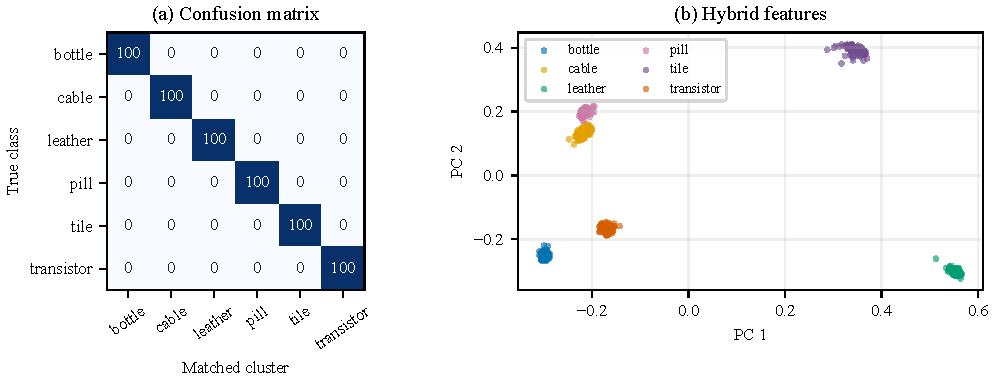
\includegraphics[width=.82\textwidth]{cluster_diagnostics}
 \caption{混淆矩阵与融合特征的 PCA 投影。散点颜色按事后匹配的簇名称标注}
 \Description{The confusion matrix contains six diagonal cells of 100. The first two principal components display the 600 images coloured by cluster.}
 \label{fig:cluster-results}
\end{figure*}

表\ref{tab:clustering}中的各方法给出同一划分，说明本数据中的形状、背景和纹理已形成很强的类别差异。图\ref{fig:cluster-exemplars}给出每簇靠近融合特征中心的图像。电缆、瓶口和药片有不同的主体轮廓，皮革和瓷砖则在色彩及细纹上有明显区别。手工特征 K-means 因此也是这个数据集上的低成本方案。本实验使用题目给定的 $K$，结果反映对这 600 张图像的聚类质量。是否能自动发现类别数，或处理背景变化和外观相近的产品，有待额外数据检验。

\begin{figure*}[t]
 \centering
 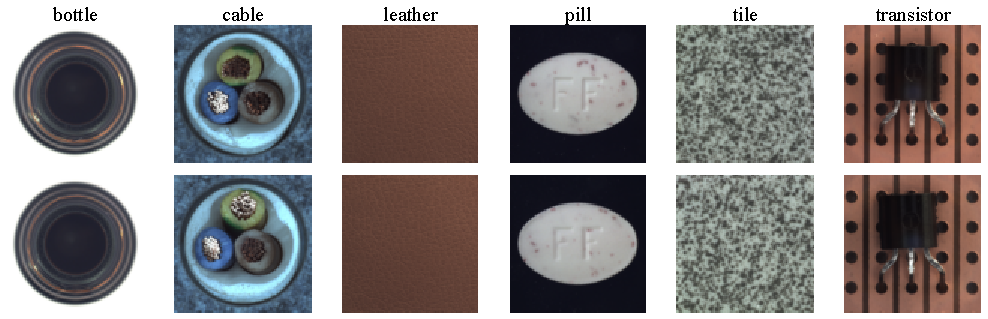
\includegraphics[width=.81\textwidth]{cluster_exemplars}
 \caption{每个簇中距其融合特征中心最近的两张图像}
 \Description{Two images each of bottles, cables, leather, pills, tiles, and transistors.}
 \label{fig:cluster-exemplars}
\end{figure*}

